\chapter{The Compact Muon Solenoid Detector}
\label{chap:CMS}

The \ac{CMS} detector~\cite{CMS:2008xjf} is one of the two general-purpose detectors involved in the discovery of the Higgs boson in 2012~\cite{ATLAS:2012yve,CMS:2012qbp}. It is located around 100 meters underground near the French town of Cessy. The full detector weights over 14 thousand tones, and is roughly cylindrically symmetric with a length and diameter of 21 and 15 meters, respectively. It consists of several layers of subsystems, as illustrated in Figure~\ref{fig:CMS}.

\begin{figure}[tbh!]
 \begin{center}
 \begin{tabular}{c}
 \includegraphics[width=0.8\textwidth]{figures/Part2/CMS/cms}
 \end{tabular}
 \caption{A sectional view of the \ac{CMS} detector, adapted from~\cite{Sakuma:2013jqa}.}
 \label{fig:CMS}
 \end{center}
\end{figure}

Brief descriptions of these subsystems are given in \autoref{sec:TK}-\autoref{sec:TrigSys}. The coordinate system adopted by \ac{CMS} is introduced in \autoref{sec:Coord}.

\section{Coordinate System Used in the CMS Detector}
\label{sec:Coord}

As illustrated in Figure~\ref{fig:axis3D}, the coordinate system adopted by \ac{CMS} uses the nominal \ac{IP} as its origin, with the x-axis pointing radially inward towards the center of the \ac{LHC} ring, the y-axis pointing vertically upward towards the sky, and the z-axis pointing along the beam line towards west of the detector.

\begin{figure}[tbh!]
 \begin{center}
 \begin{tabular}{c}
 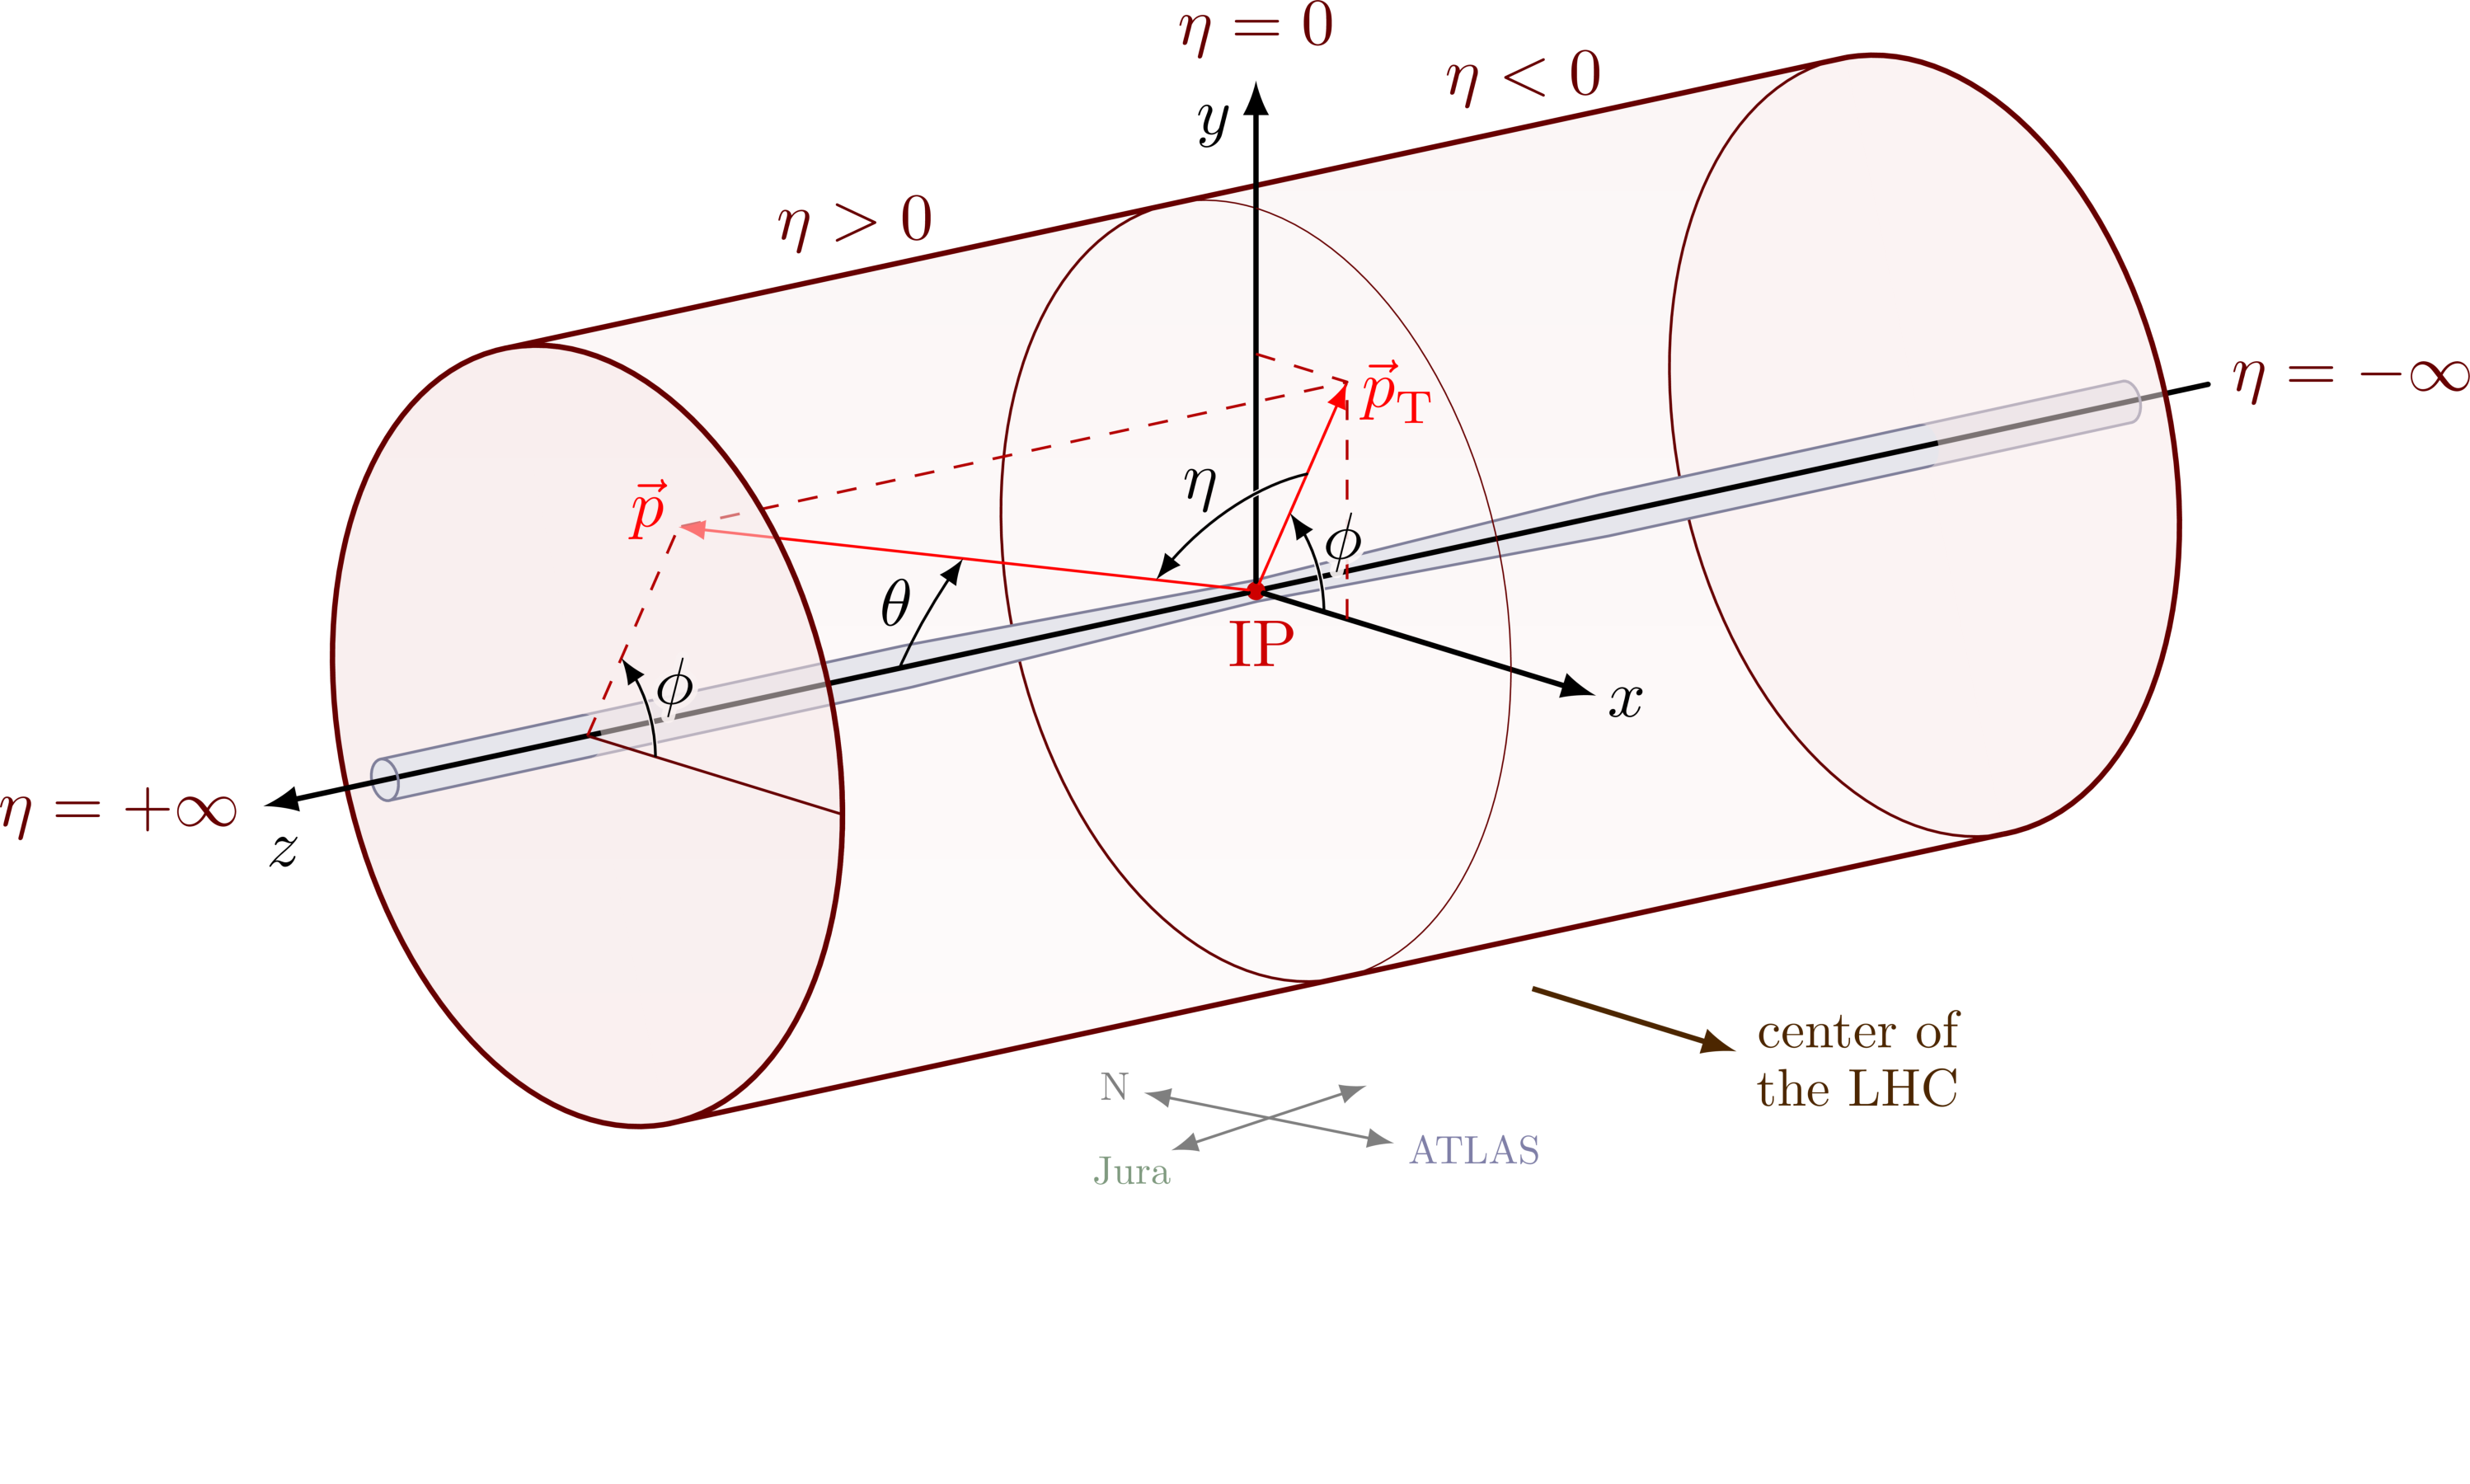
\includegraphics[width=0.8\textwidth]{figures/Part2/CMS/axis3D_CMS-004}
 \end{tabular}
 \caption{A sketch of the coordinate system adopted by \ac{CMS}, adapted from~\cite{tikz:3D}.}
 \label{fig:axis3D}
 \end{center}
\end{figure}

The x- and y-axis form the transverse plane as they are both orthogonal to the beam line (z-axis). The distance from the \ac{IP} in the transverse plane is defined as $r=\sqrt{x^2+y^2}$. Variables defined entirely in the transverse plane, such as $\pt$, \MET, and $\Ht$, are often indicated by a subscripted T. The azimuthal angle $\phi$ is measured from the positive x-axis and the polar angle $\theta$ is measured from the positive z-axis. Another variable $\eta$, known as pseudorapidity, is defined as

\begin{equation}
\eta=-\ln(\frac{\theta}{2}).
\end{equation}

It is preferred over $\theta$ mainly due to: i) particle production rate is roughly uniform in this variable, and ii) a difference in this variables, denoted by $\mathrm{\Delta}\eta$, is invariant under Lorentz boosts. The conversion between $\eta$ and $\theta$ is illustrated in Figure~\ref{fig:axis2D}. The $\mathrm{\Delta}\eta$ and the difference in azimuthal angles, denoted by $\mathrm{\Delta}\phi$, are used to define the distance parameter $\mathrm{\Delta}R$

\begin{equation}
\label{eq:DR}
\mathrm{\Delta}R=\sqrt{\mathrm{\Delta}\eta^2+\mathrm{\Delta}\phi^2}.
\end{equation}

\begin{figure}[tbh!]
 \begin{center}
 \begin{tabular}{c}
 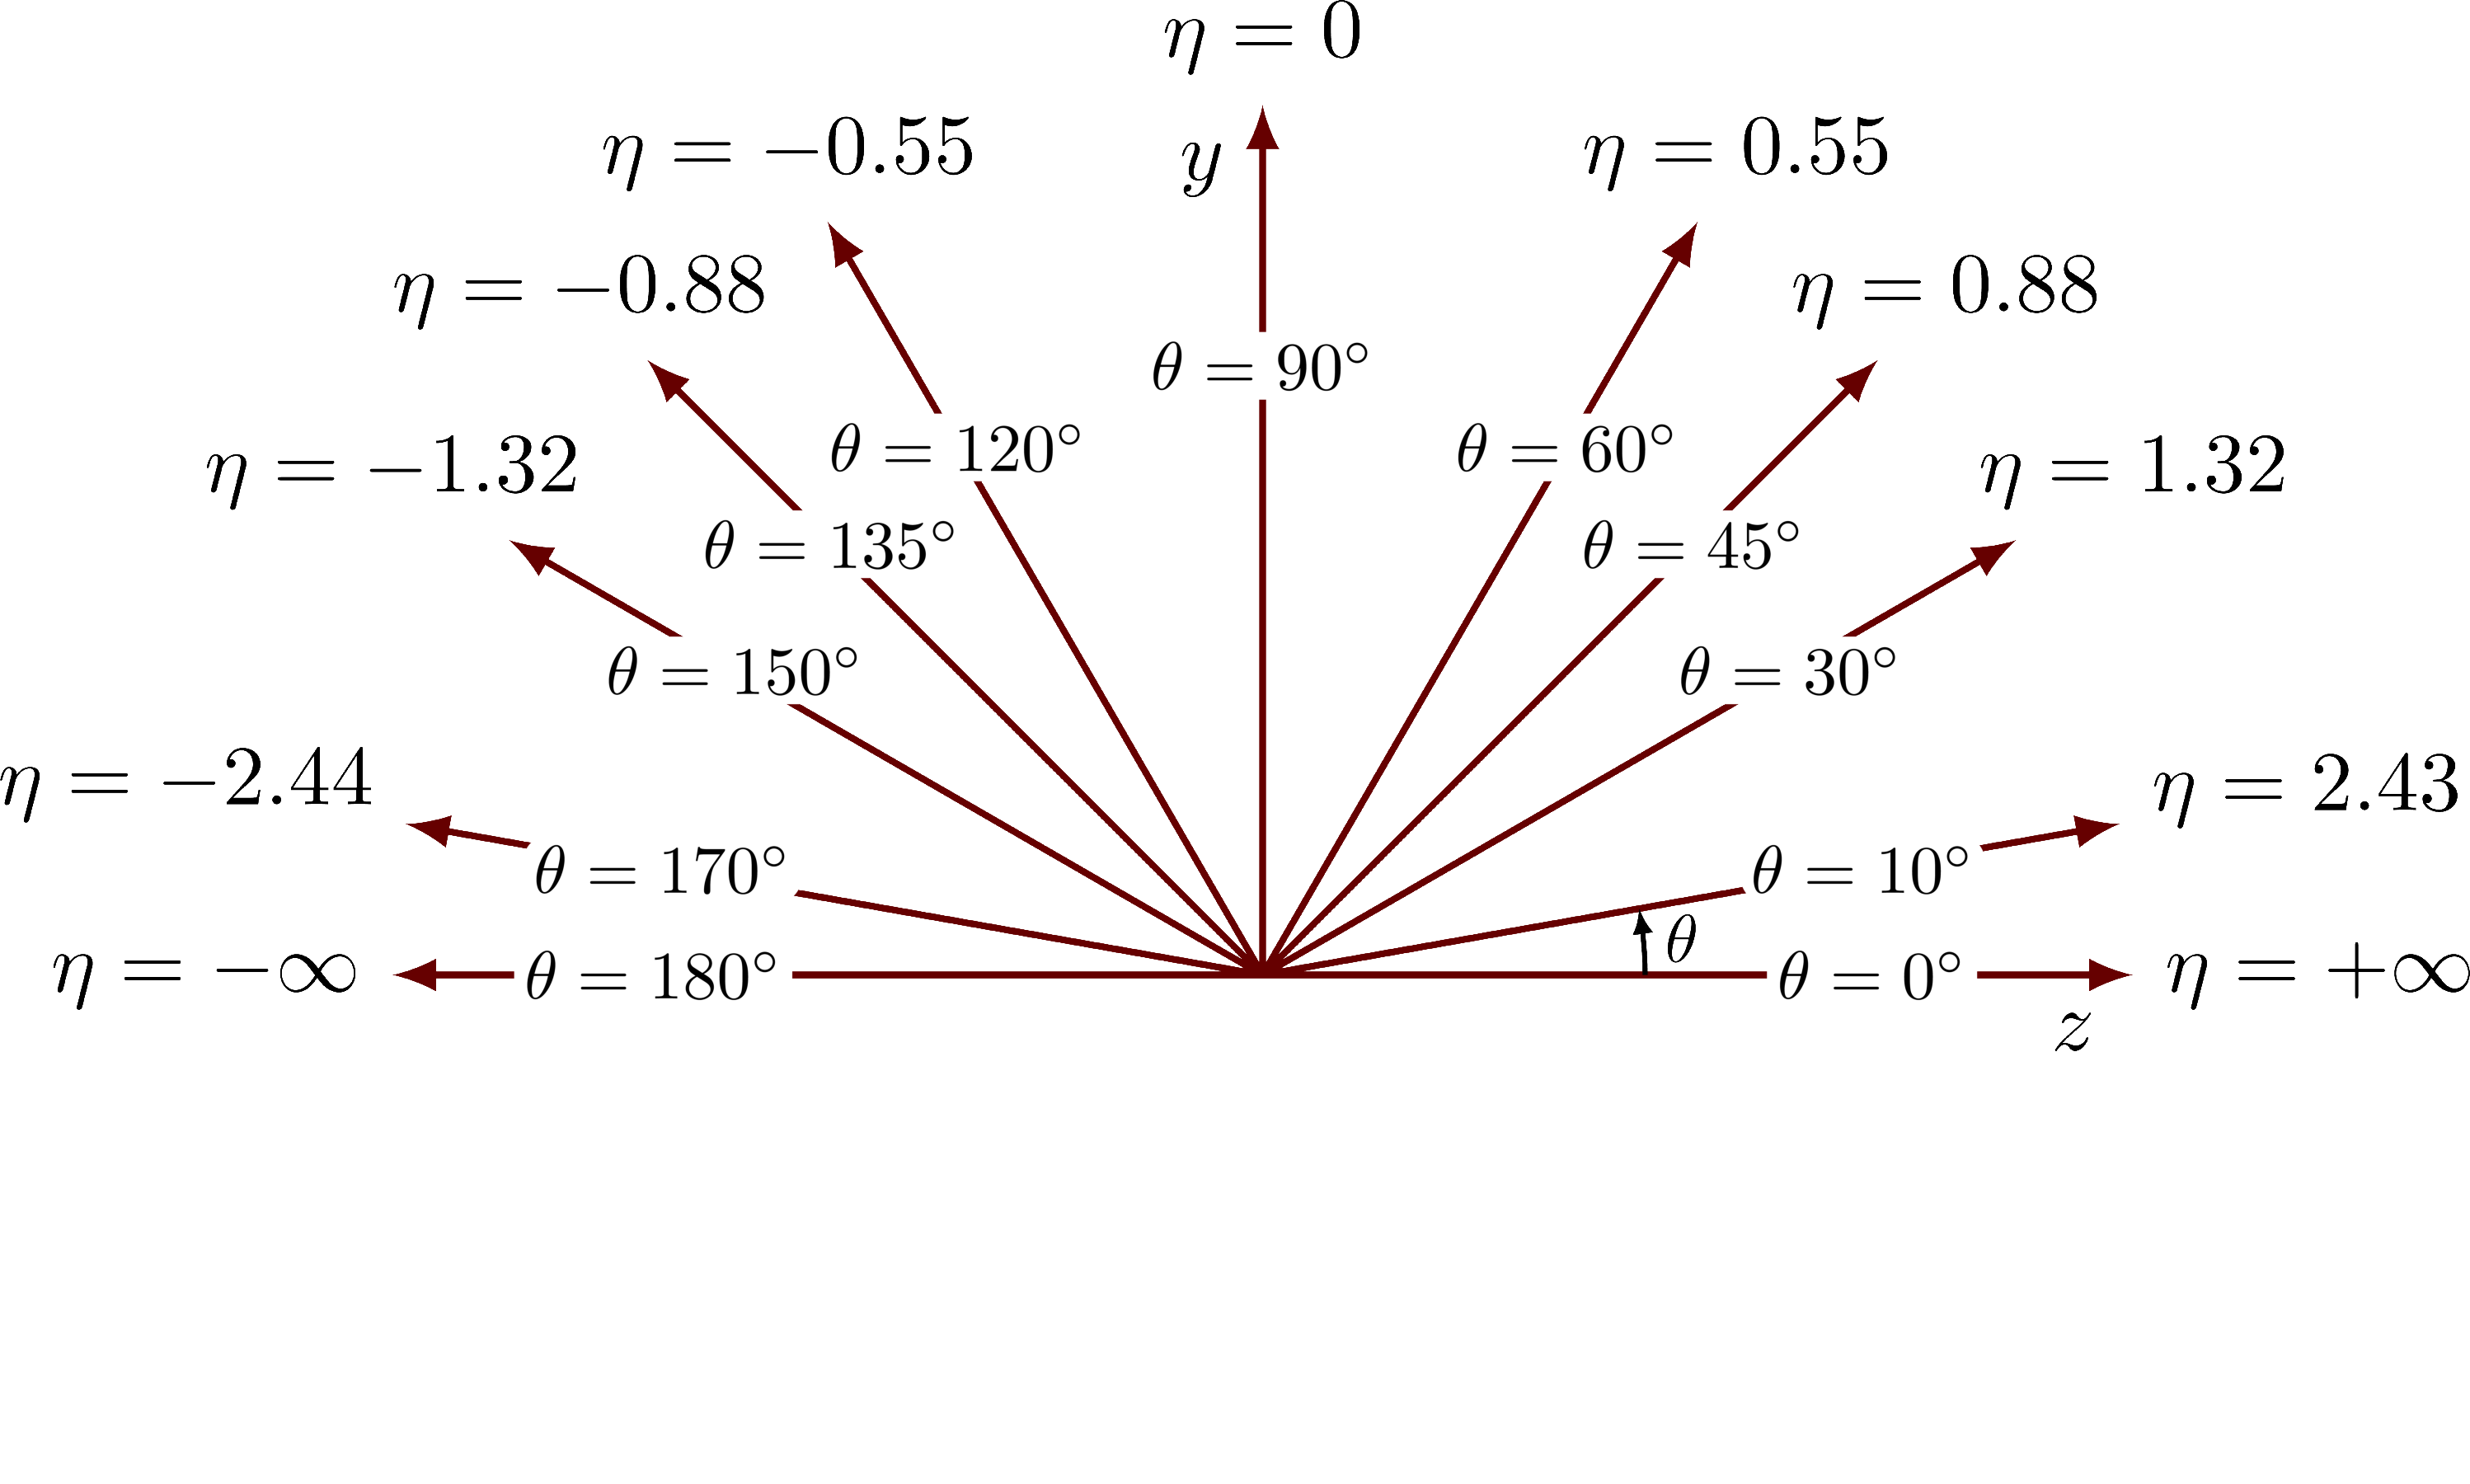
\includegraphics[width=0.8\textwidth]{figures/Part2/CMS/axis2D_pseudorapidity-003}
 \end{tabular}
 \caption{Examples of the conversion between the polar angle $\theta$ and the pseudorapidity $\eta$, adapted from~\cite{tikz:2D}.}
 \label{fig:axis2D}
 \end{center}
\end{figure}

\section{The Tracking System}
\label{sec:TK}

The tracking system~\cite{CMS:1997tlf} is the innermost subsystem of the \ac{CMS} detector where the density of particles from the collisions is the highest. The full tracking system is based on silicon technology to cope with the high radiation condition and provide excellent spatial resolutions while maintaining a light material budget. Hits from charged particles, such as electrons and muons, are measured by silicon sensors and used reconstruct particle trajectories, known as ``tracks''. The curvature of tracks can be then used to determine the momentum of these final state particles. Tracks can also be used to reconstruct the \ac{PV}, which corresponds to the hard scattering in collision events, and the \ac{SV}, which corresponds to the decay of heavy particles, such as tau leptons. 

The tracking system gives a coverage of up to $|\eta|~<$ 2.5, and is comprised of a pixel detector and a strip detector, which are also collectively known as the tracker detector. When charged particles go through tracker layers, they knocked out electrons in detector materials. These electrons create electric pulses when they travel in electric fields, which are then amplified and detected in the readout electronics. A sketch of the \ac{CMS} tracker created shortly before Run-1 of the \ac{LHC} is shown in Figure~\ref{fig:Tracker}.

\begin{figure}[tbh!]
 \begin{center}
 \begin{tabular}{c}
 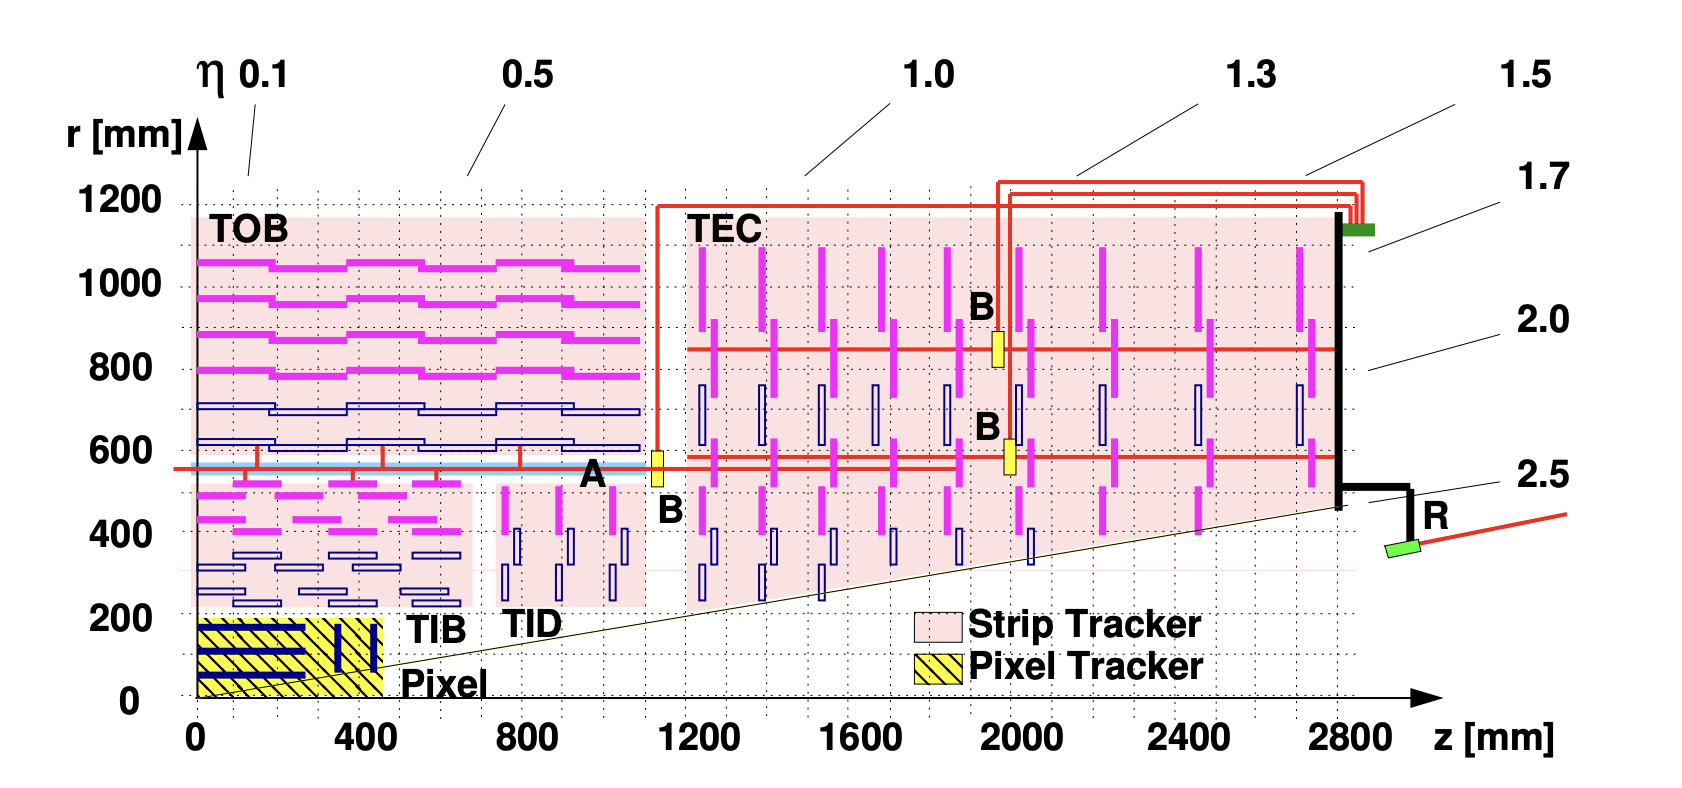
\includegraphics[width=0.8\textwidth]{figures/Part2/CMS/Tracker}
 \end{tabular}
 \caption{Layout of one quadrant of the \ac{CMS} tracker in the $r-z$ plane, adapted from~\cite{CMS:2009dvy}. The strip tracker is shown in pink color while the original pixel detector with three barrel layers is shown in black color.}
 \label{fig:Tracker}
 \end{center}
\end{figure}

The pixel tracker is comprised of roughly 66 million silicon sensors~\cite{CMS:2014pgm}, and is divided into two subsystems: the Barrel Pixel (BPIX) and  Forward Pixel (FPIX). The BPIX is composed of three cylindrical layers with radii ranging from 44 mm to 102 mm. The FPIX is composed of two disks on each side of the forward region. To cope with the intensified \ac{LHC} conditions in Run-2 and improve the overall tracking performance, an upgraded version of the pixel detector, referred to as the Phase-1 pixel detector, was installed during the year-end technical stop between 2016 and 2017~\cite{CMSTrackerGroup:2020edz}. The Phase-1 pixel detector is comprised of roughly 124 million silicon sensors distributed over four BPIX layers and three FPIX disks on each side. Differences between the two pixel detectors are shown in Figure~\ref{fig:Pixel}.

\begin{figure}[tbh!]
 \begin{center}
 \begin{tabular}{c}
 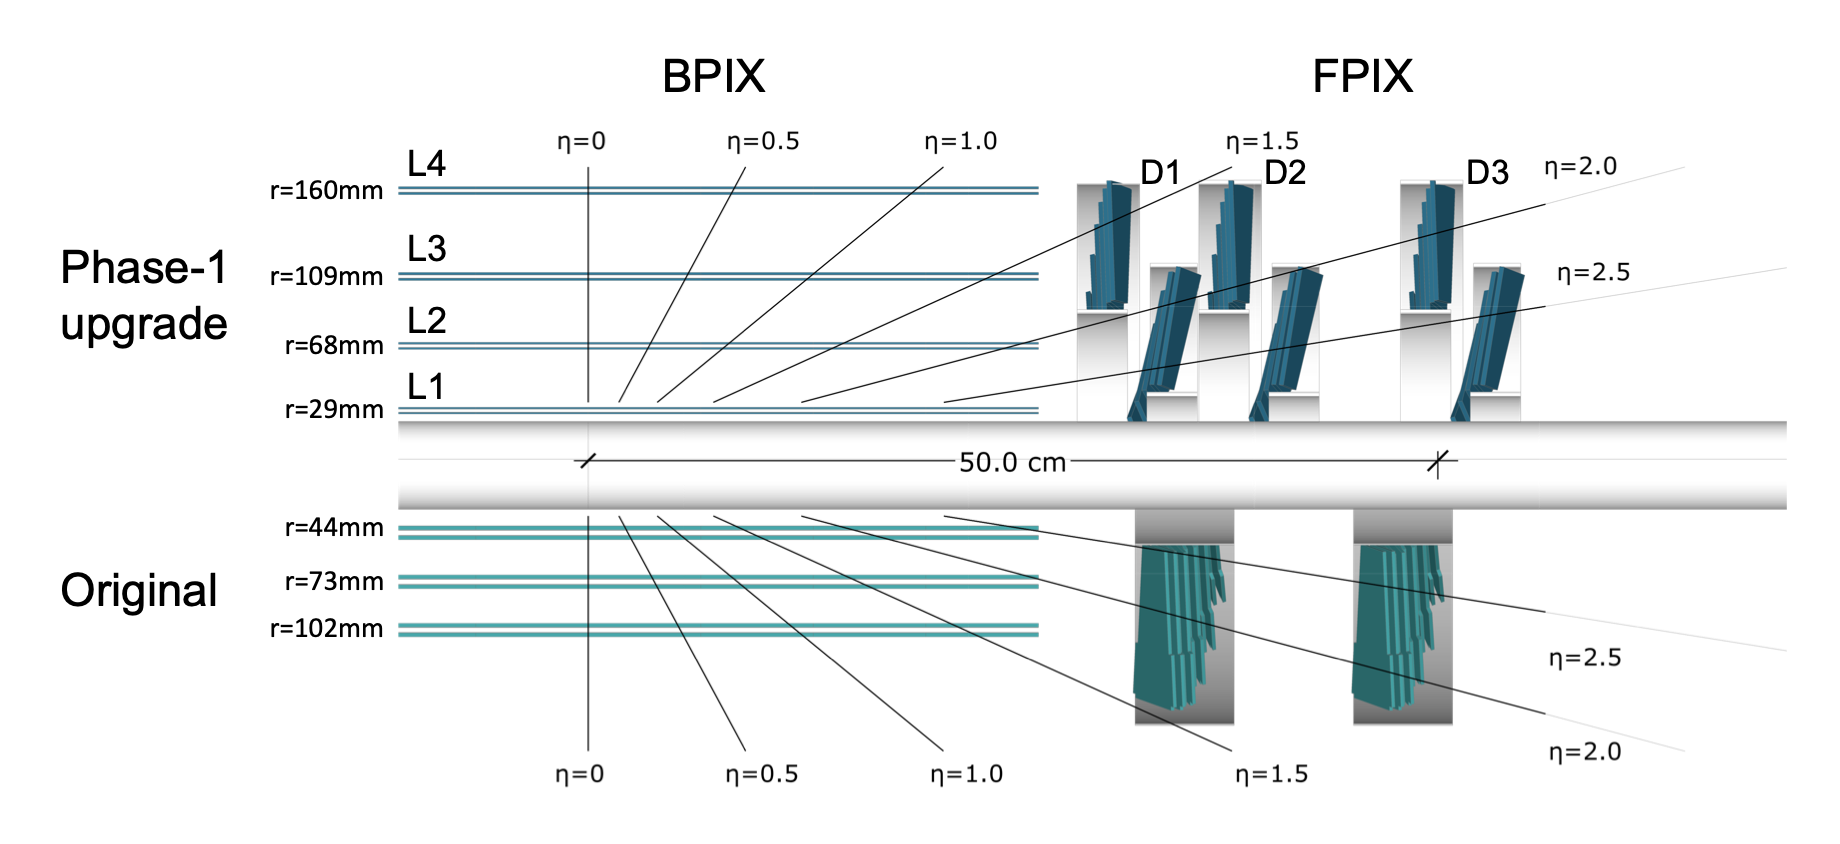
\includegraphics[width=0.8\textwidth]{figures/Part2/CMS/Pixel}
 \end{tabular}
 \caption{A comparison between the original pixel detector and the upgraded pixel detector in the $r-z$ plane, adapted from~\cite{CMSTrackerGroup:2020edz}.}
 \label{fig:Pixel}
 \end{center}
\end{figure}

The strip tracker is much larger in size and is built around the pixel tracker. It is comprised of roughly 10 million silicon sensors and is divided into several subsystems: the Tracker Inner Barrel (TIB), Tracker Outer Barrel (TOB), Tracker Inner Disks (TID), and Tracker Endcaps (TEC). The TIB and TOB consist of four and six layers, respectively. The TID and TEC consist of three and nine disks, respectively.

\section{The Electromagnetic Calorimeter}
\label{sec:ECAL}

The \ac{ECAL}~\cite{CMS:1997ysd} encloses the tracker detector and is the second innermost subsystem of the \ac{CMS} detector. It helps determine the energy and position of electrons and photons through their electromagnetic interactions with detector materials. The \ac{ECAL} gives a coverage of up to $|\eta|~<$ 3.0, and is divided into three subsystems: the \ac{ECAL} Barrel (EB), \ac{ECAL} Preshower (ES), and \ac{ECAL} Endcap (EE). A sketch of the \ac{ECAL} layout is shown in Figure~\ref{fig:ECAL}.

\begin{figure}[tbh!]
 \begin{center}
 \begin{tabular}{c}
 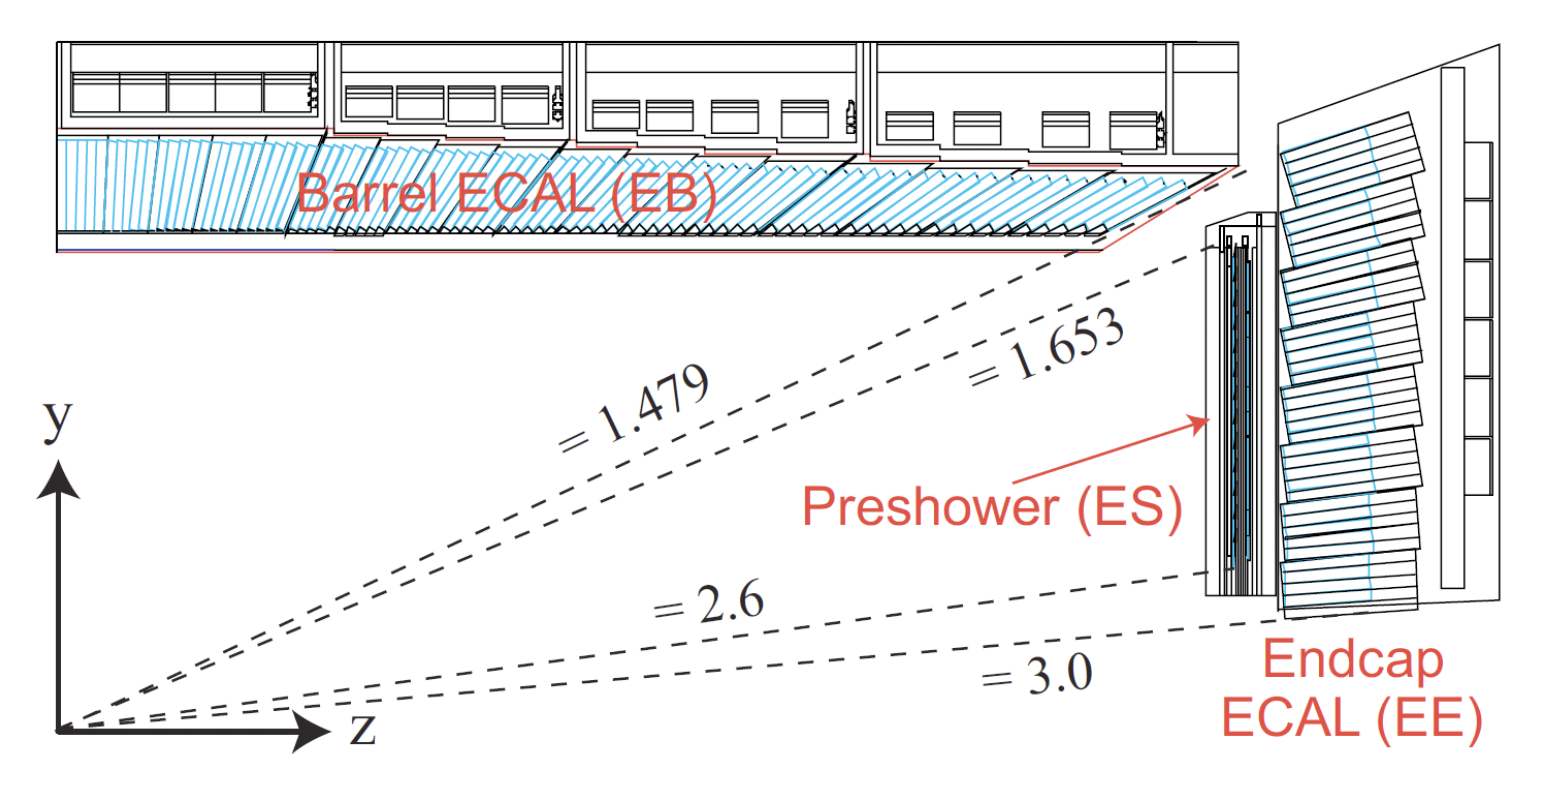
\includegraphics[width=0.8\textwidth]{figures/Part2/CMS/ECAL}
 \end{tabular}
 \caption{Layout of one quadrant of the \ac{ECAL} in the $r-z$ plane, adapted from~\cite{Benaglia:2014aqa}.}
 \label{fig:ECAL}
 \end{center}
\end{figure}

The \ac{ECAL} is composed of over 76 thousand lead tungstate (PbWO$_{4}$) crystals, which act as absorber and scintillator simultaneously. Electrons and photons create electromagnetic showers when they travel through these crystals. Over 98 \% of the shower energy can be absorbed and converted to light through the scintillation process. The scintillation light is then amplified and detected by photodiodes. The energy of particles can be measured from the intensity of the scintillation light.

\section{The Hadronic Calorimeter}
\label{sec:HCAL}

The \ac{HCAL}~\cite{CMS:1997xji} consists of multiple layers of tiles that form a closed space to ensure high efficiency of missing transverse energy measurement of invisible particles. The tiles stop hadrons completely and transfer the signals to reconstruct the energy and positions of particles.

\section{The Superconducting Magnet}
\label{sec:Magnet}

The superconducting solenoid~\cite{CMS:1997moj} produces a magnetic field that is close to 4T. The paths of charged particles are curved by this magnetic field in order to identify the charge and momentum of particles. A strong magnetic field is able to curve particles with high energy and provides a good resolution in the high transverse momentum region.

\section{The Muon System}
\label{sec:MuonSys}

The muon detector~\cite{CMS:1997iti} is the outermost detector of the CMS. The \ac{DT} and \ac{RPC} together make up the barrel region of the muon system, and the end-cap muon system consists of \ac{RPC} and  \ac{CSC}. The \ac{GEM} is the latest addition to the muon system. It complements \ac{CSC} in the forward region. The muon system reconstructs the tracks of muons, and with the strong magnetic field produced by the superconducting solenoid and its iron flux return, the tracks are bent in order to calculate the momentum of muons.

\section{The Trigger System}
\label{sec:TrigSys}

\ac{L1} \ac{HLT} 